\documentclass{article}
\usepackage[utf8]{inputenc}
\usepackage{ragged2e}
\usepackage{latexsym}
\usepackage{graphicx}
\usepackage{url}
\usepackage{cite}

\title{Combinatorial Optimization by Shortest Path Algorithms}
\author{Kim Hue Nguyen, Ngoc Lich Dang, Huu Loi Nguyen}
\date{April 2019}

\begin{document}

\maketitle
\begin{quote}
    \textbf{Abstract} : Nowadays, in computer networks, the routing is based on the shortest path problem. This will help in minimizing the overall costs of setting up computer networks. New technologies such as map-related systems are also applying the shortest path problem. This paper’s main objective is to develop an algorithm based on solving the combinatorial optimization to find the shortest path on a network.
    \vspace{10pt}
    \\
    \textbf{Index Terms} : shortest path problem
\end{quote}

\section{Introduction}

The shortest path problem is a problem of finding the shortest path or route from a starting point to a final destination. Generally, in order to represent the shortest path problem we use graphs. A graph is a mathematical abstract object, which contains sets of vertices and edges. Edges connect pairs of vertices. Along the edges of a graph it is possible to walk by moving from one vertex to other vertices. Depending on whether or not one can walk along the edges by both sides or by only one side determines if the graph is a directed graph or an undirected graph. In addition, lengths of edges are often called weights, and the weights are normally used for calculating the shortest path from one point to another point. For example, in order to represent a map we can use a graph, where vertices represent cities and edges represent routes that connect the cities. If routes are one-way then the graph will be directed; otherwise, it will be undirected. There exist different types of algorithms that solve the shortest path problem: Dijkstra’s Algorithm, Floyd-Warshall Algorithm, Bellman-Ford Algorithm, Genetic Algorithm… 
\vspace{5pt}
\\
In graphs, the distance between two nodes s and t (source and target, respectively) is defined as follows. If s and t are connected by an edge, their distance is 1. If they are not directly connected, the distance is defined by the length of a shortest path between s and t, which is a sequence of adjacent edges. In a weighted graph, the length of a path is defined by the sum of the weights of the edges on the path. Consequently, shortest paths are defined with respect to these weights. Note that, in weighted graphs, even if two nodes are connected by an edge, depending on its weight, the edge is not necessarily part of any shortest path.
\vspace{5pt}
\\
So far, in the new graph only consider the weights of the edges, the vertices independently, in which the length of the path is merely the sum of the weights of the edges and vertices on that path. However, in many practical problems, the weight at a vertex is not the same for every path that passes that peak, but also depends on the edge going to and from the top. In the paper, the general graph model is defined. This paper’s main objective is to develop and demonstrate the algorithm to find the shortest path between two peaks and the algorithm to find the shortest path from one peak to the other peaks on the general transport network.
\vspace{5pt}
\\
In this paper, we will use Dijkstra’s Algorithm to solve the shortest path problem.

\section{Related Work}

\begin{itemize}
\item Implement the algorithm that can be adaptive to any input data change.
\item Read input data from the nodes and edges, and predict the shortest path
\item Design the interface for input from user by representing the feature like: Add, Insert, Delete, Dropout, Change parameters, ... 
\item Visualize the networks
\end{itemize}

\section{Approaches}

As mentioned earlier, a graph can be used to represent a map where the cities are represented by vertices and the routes or roads are represented by edges within the graph. In this section, a graph representation of a map is explained further, and brief descriptions and implementations of Dijkstra’s Algorithm being studied are presented.
\vspace{5pt}
\\
The distance between two nodes \textit{s}, \textit{t} $\in$ V of a graph G = (V, E) is defined by the length of a shortest path. The objective is to find the shortest possible path that connects the source and the target. For each vertex within a graph we assign a label that determines the minimal length from the starting point \textit{s} to other vertices \textit{v} of the graph. In a computer we can do it by declaring an array \textit{d[]}. The algorithm works sequentially and in each step it tries to decrease the value of the label of the vertices. The algorithm stops when all vertices have been visited. The label at the starting point \textit{s} is equal to zero (\textit{d[s] = 0}); however, labels in other vertices v are equal to infinity \textit{(d[v] = $\infty$)}, which means that the length from the starting point \textit{s} to other vertices is unknown. In a computer we can just use a very big number in order to represent infinity. 
\vspace{5pt}
\\
In addition, for each vertex \textit{v} we have to identify whether it has been visited or not. In order to do that, we declare an array of Boolean type called \textit{u[v]}, where initially, all vertices are assigned as unvisited (\textit{u[v] = false}). The Dijkstra’s algorithm consists of n iterations. If all vertices have been visited, then the algorithm finishes; otherwise, from the list of unvisited vertices we have to choose the vertex which has the minimum (smallest) value at its label (At the beginning, we will choose a starting point s). After that, we will consider all neighbors of this vertex (Neighbors of a vertex are those vertices that have common edges with the initial vertex). For each  unvisited neighbor we will consider a new length, which is equal to the sum of the label’s value at the initial vertex \textit{v} (\textit{d[v]}) and the length of edge l that connects them. If the resulting value is less than the value at the label, then we have to change the value in that label with the newly obtained value [1].

\begin{equation}
    d [ neighbors ] = min ( d [ neighbors ] ,  d[ v ]  +  l )       
\end{equation}
\\
After considering all of the neighbors, we will assign the initial vertex as visited (\textit{u[v] = true}). After repeating this step n times, all vertices of the graph will be visited and the algorithm finishes or terminates. The vertices that are not connected with the starting point will remain by being assigned to infinity. In order to restore the shortest path from  the starting point to other vertices, we  need to identify array \textit{p[]}, where for each vertex, where \textit{v} $\neq$ \textit{s}, we will store the number of vertex \textit{p[v]}, which penultimate vertices in the  shortest  path. In other words, a complete path from \textit{s} to \textit{v} is equal to the following statement [3]

\begin{equation}
   P = ( s , … , p [ p [ p [ v ] ] ] , p [ p [ v ] ] , p [ v ] , v )      
\end{equation}
\\
When planning a route, it is actually not necessary to wait until the destination node is "visited" as above: the algorithm can stop once the destination node has the smallest tentative distance among all "unvisited" nodes (and thus could be selected as the next "current").
\vspace{5pt}
\\
In the following algorithm, we have the pseudocode of Dijkstra’s algorithm. The code \textit{u} $\leftarrow$ vertex in \textit{Q} with min dist[\textit{u}], searches for the vertex \textit{u} in the vertex set \textit{Q} that has the least dist[\textit{u}] value, length(\textit{u,v}) returns the length of the edge joining (i.e. the distance between) the two neighbor-nodes \textit{u} and \textit{v}. The variable \textit{alt} on line 18 is the length of the path from the root node to the neighbor node \textit{v} if it were to go through \textit{u}. If this path is shorter than the current shortest path recorded for \textit{v}, that current path is replaced with this \textit{alt} path. The prev array is populated with a pointer to the "next-hop" node on the source graph to get the shortest route to the source.
\vspace{5pt}
\\

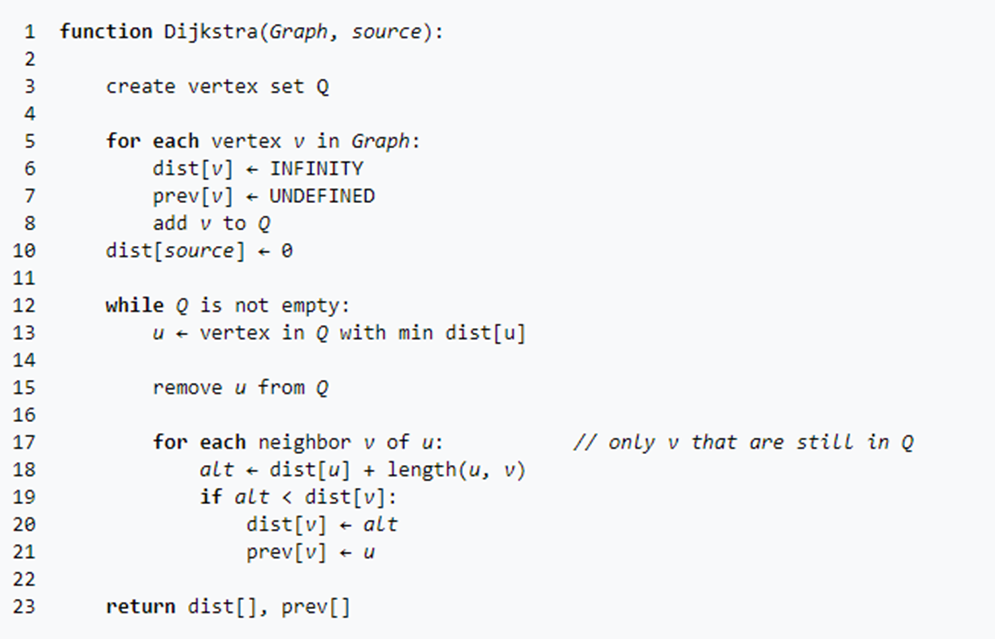
\includegraphics[width=320pt]{image/Pseudocode.png}
\begin{center}
    \textbf{Figure 3.1}: \textit{Pseudocode of Dijkstra’s algorithm}
\end{center}
\begin{flushright}
    (Source: Pseudocode of Dijkstra’s Algorithm\\
    Available at \url{https://en.wikipedia.org/wiki/Dijkstra%27s_algorithm}) 
\end{flushright}

When the algorithm completes, \textit{prev[]} data structure will actually describe a graph that is a subset of the original graph with some edges removed. Its key property will be that if the algorithm was run with some starting node, then every path from that node to any other node in the new graph will be the shortest path between those nodes in the original graph, and all paths of that length from the original graph will be present in the new graph. Then to actually find all these shortest paths between two given nodes we would use a path finding algorithm on the new graph, such as depth-first search.

\section{Experiments and Results}

\begin{center}
    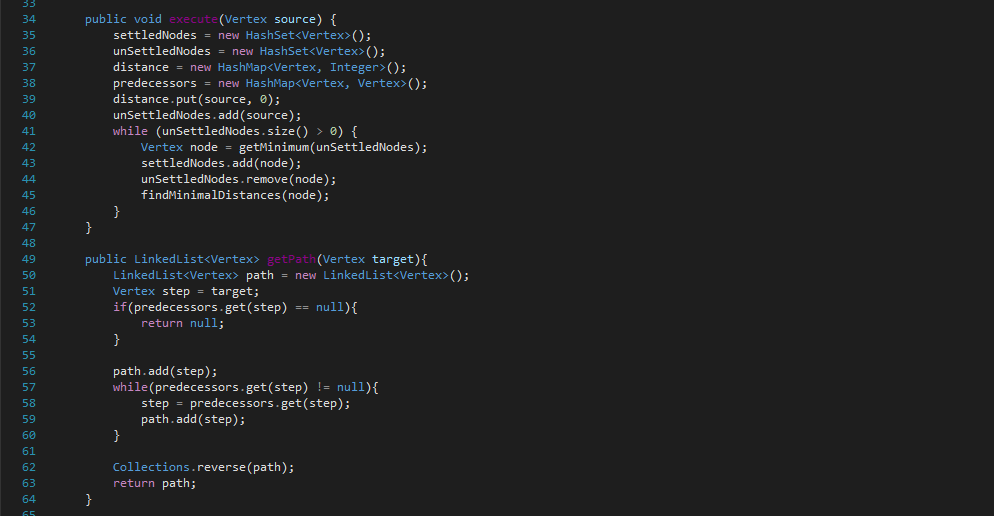
\includegraphics[width=320pt]{image/1.png}
    \textbf{Figure 4.1}: \textit{Execute and get path}
    \begin{flushright}
        (Source: DijkstraAlgorithm.java) 
    \end{flushright}
\end{center}

\begin{center}
    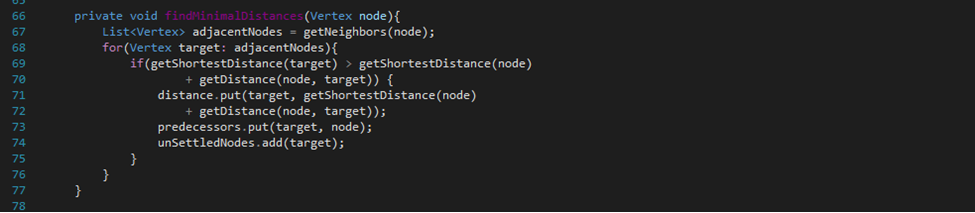
\includegraphics[width=320pt]{image/2.png}
    \textbf{Figure 4.2}: \textit{Minimal Distances}
    \begin{flushright}
        (Source: DijkstraAlgorithm.java) 
    \end{flushright}
\end{center}

\begin{center}
    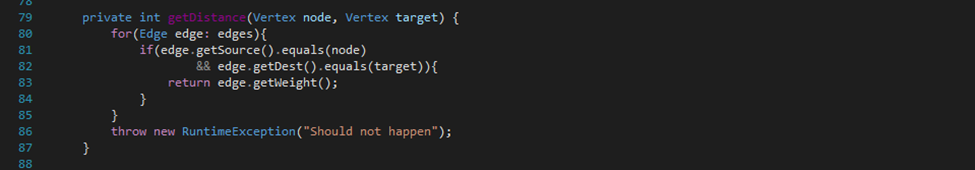
\includegraphics[width=320pt]{image/3.png}
    \textbf{Figure 4.3}: \textit{Get Distance}
    \begin{flushright}
        (Source: DijkstraAlgorithm.java) 
    \end{flushright}
\end{center}

\begin{center}
    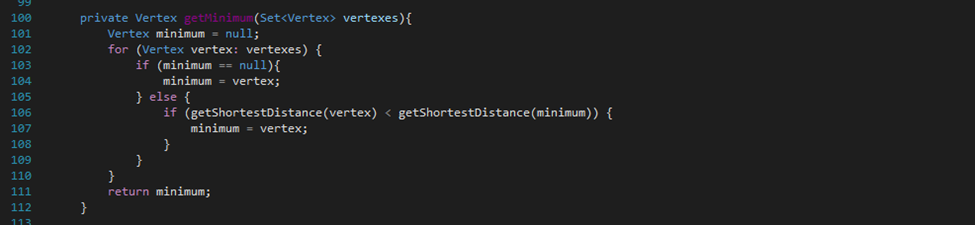
\includegraphics[width=320pt]{image/4.png}
    \textbf{Figure 4.4}: \textit{Get Minimum}
    \begin{flushright}
        (Source: DijkstraAlgorithm.java) 
    \end{flushright}
\end{center}
\vspace{5pt}
The time complexity for Dijkstra’s algorithm is illustrated in Table I; n represents the total number of vertices, and m is the total number of edges.  

\begin{table}[!th]
    \centering
    \begin{tabular}{c|c|c}
         &  Algorithm & Time complexity\\
         & Dijkstra & $n^{2}+m$
    \end{tabular}
    \textsc{\caption{TIME COMPLEXITY}}
    \label{tab:my_label}
\end{table}

\section{Conclusion}

The computed time complexity for each of the Dijkstra’s algorithm show that the algorithm is acceptable in terms of the overall performance in solving the shortest path problem. Nowadays, there are also many intelligent shortest path algorithms that have been introduced in several past research papers. For example, the authors in "A  New  Shortest Path Algorithm based on Heuristic Strategy" used a heuristic method for  computing the shortest path from one point to another point within traffic networks. They proposed a “new dynamic direction restricted algorithm obtained by extending the Dijkstra’s algorithm.” In addition, other artificial intelligence techniques such as fuzzy logic and neural networks can also be implemented in improving existing shortest path algorithms in order to make them more intelligent and more efficient.

\begin{thebibliography}{}

    \bibitem{1} M.Jordan, {\it “Notes 7 for CS170”}, UC Berkeley, 2005.
    \bibitem{2} M.Kairanbay, Hajar Mat Jani, {\it A Review And Evaluations Of Shortest Path Algorithms”}, 2013.
    \bibitem{3} J.Chamero, {\it “Dijkstra’s Algorithm”}, Discrete Structures \& Agorithms, 2006.
    \bibitem{4} MDijkstra’s Algorithm, Available at \url{https://en.wikipedia.org/wiki/Dijkstra%27s_algorithm} 
\end{thebibliography}

\end{document}
